\message{ !name(chapter2_3.tex)}\documentclass{report}

\usepackage{subcaption} % package for subfigures
\usepackage{hyperref}  % package for linking figures etc
\usepackage{enumitem}  % package for description with bullets
\usepackage{graphicx}  % package for importing images
\usepackage{mathtools} % package for math equation
\usepackage{mathrsfs}  % package for math font
\usepackage{indentfirst} % package for getting ident after section or paragraph
\usepackage{amssymb}
% \usepackage{amsmath}
\usepackage[
    backend=bibtex,
    citestyle=authoryear,
    % citestyle=authoryear-comp,
    % citestyle=authoryear-ibid,
    bibstyle=numeric,
    sorting=ynt,
    % style=numeric,
    % style=alphabetic ,
  ]{biblatex}
 
 \addbibresource{References}


\setlength{\parindent}{2em} % how much indent to use when we start a paragraph

\graphicspath{ {./theory/figures/} }       % path for images

\begin{document}

\message{ !name(chapter2_3.tex) !offset(-3) }


\chapter{Background}


\section{Machine Learning}

\subsection{Introduction}
Machine Learning (ML) is a field which is raised out of Artificial Intelligence (AI). Applying AI, we wanted to build better and intelligent
machines. But except for mere tasks such as finding the shortest path between point A and B, we were unable to program more complex
and constantly evolving challenges. There was a realization that the only way to be able to achieve this task was to let machines learn
from themselves. This sounds similar to a child learning from its self. So machine learning was developed as a new capability for computers.
And now machine learning is present in so many segments of technology, that we don’t even realize it while using it. \par
Finding patterns in data on planet earth is possible only for human brains. Data being very massive and time taken to compute them made  Machine Learning take  action, in order to help people exploit them in minimum time. \\
There are three kinds of Machine Learning Algorithms :
 
\begin{enumerate}
\item Supervised Learning
\item Unsupervised Learning
\item Reinforcement Learning
\end{enumerate}

\subsubsection{Supervised Learning}
A majority of practical machine learning uses supervised learning. In supervised learning, the system tries to learn from the previous examples that are given. Speaking mathematically, supervised learning is where you have both input variables (\textit{x}) and output variables (\textit{Y}) and can use an algorithm to derive the mapping function from the input to the output. The mapping function is expressed as
$Y = f(x)$.
\begin{figure}[h]
  \centering
  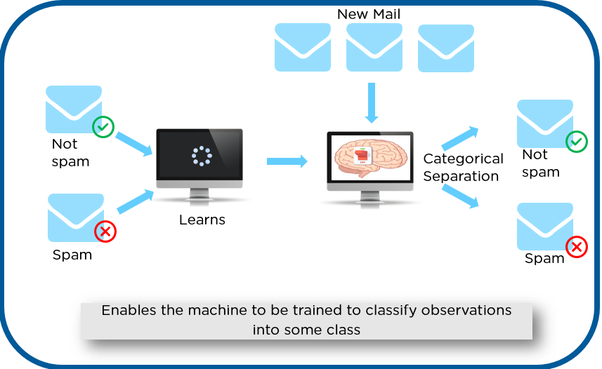
\includegraphics[scale=0.3]{supervised_leaning_example2}
  \caption{Example of supervised Learning}
  \label{fig:supervised_learning_example}
\end{figure}

As shown in Figure \ref{fig:supervised_learning_example}, we have initially taken some data and marked them as ‘Spam’ or ‘Not Spam’. This
labeled data is used by the training supervised model, in order to train the model. Once it is trained, we can test our model by testing it with some new mails and checking if the model is able to predict the right output. 

Supervised learning problems can be further divided into two parts, namely \textbf{classification}, and \textbf{regression}.
\begin{description}
\item[ Classification] : A classification problem is when the output variable is a category or a group, such as “black” or “white” or “spam” and “no spam”.
\item[ Regression ] :  A regression problem is when the output variable is a real value, such as “Rupees” or “height.”
\end{description}
Some Supervised learning algorithms include:
\begin{itemize}
\item Decision trees
\item Support-vector machine
\item Naive Bayes classifier
\item k-nearest neighbors
\item linear regression
\end{itemize}

\subsubsection{Unsupervised Learning}

In unsupervised learning, the algorithms are left to themselves to discover interesting structures in the data. Mathematically, unsupervised
learning is when you only have input data (\textit{X}) and no corresponding output variables. This is called unsupervised learning because
unlike supervised learning above, there are no given correct answers and the machine itself finds the answers.
\begin{figure}[h]
  \centering
  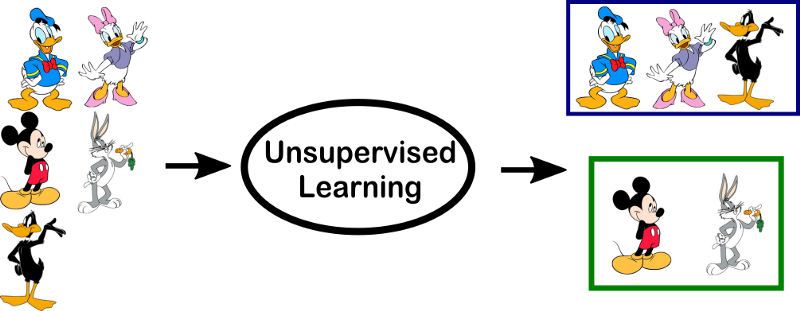
\includegraphics[scale=0.3]{unsupervised_learning_example}
  \caption{Example of unsupervised Learning}
  \label{fig:unsupervised_learning_example}
\end{figure}
In Figure \ref{fig:unsupervised_learning_example}, we have given some characters to our model which are ‘Ducks’ and ‘Not Ducks’. In our
training data, we don’t provide any label to the corresponding data. The unsupervised model is able to separate both the characters by
looking at the type of data and models the underlying structure or distribution in the data in order to learn more about it. Unsupervised
learning problems can be further divided into \textbf{association} and \textbf{clustering} problems.

\begin{description}
\item[ Association] : An association rule learning problem is where you want to discover rules that describe large portions of your data, such as “people that buy X also tend to buy Y”.
\item[ Clustering] : A clustering problem is where you want to discover the inherent groupings in the data, such as grouping customers by purchasing behaviour.
\end{description}

\subsubsection{Reinforcement Learning}
A computer program will interact with a dynamic environment in which it must perform a particular goal (such as playing a game with an
opponent or driving a car). The program is provided feedback in terms of rewards and punishments as it navigates its problem space. 
Using this algorithm, the machine is trained to make specific decisions. It works this way: the machine is exposed to an environment
where it continuously trains itself using trial and error method.
\begin{figure}[h]
  \centering
  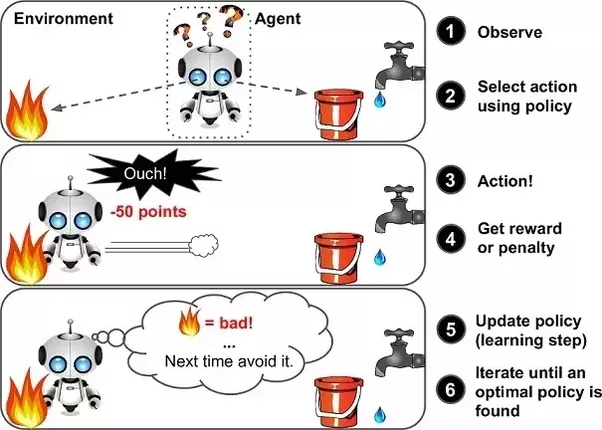
\includegraphics[scale=0.3]{reinforment_learning_example}
  \caption{Example of Reinforcement Learning}
  \label{fig:reinforment_learning_example}
\end{figure}
In Figure \ref{fig:reinforment_learning_example}, we can see that the agent is given 2 options i.e. a path with water or a path with fire. A reinforcement algorithm
works on reward a system i.e. if the agent uses the fire path then the rewards are subtracted and agent tries to learn that it should avoid
the fire path. If it had chosen the water path or the safe path then some points would have been added to the reward points, the agent then
would try to learn what path is safe and what path isn’t

\subsection{Neural Networks}
Neural Networks are a class of models within the general machine learning literature. Neural networks are a specific set of algorithms that
have revolutionized the field of machine learning. They are inspired by biological neural networks and the current so called deep neural
networks have proven to work quite very well. Neural Networks are themselves general function approximations, that is why they can be applied
to literally almost any machine learning problem where the problem is about learning a complex mapping from the input to the output space.

\subsection{A single Neuron}
The basic unit of computation in a neural network is the neuron, often called a \textbf{node} or \textbf{unit}. It receives input from some
other nodes, or from an external source and computes an output. In purely mathematical terms, a neuron in the machine learning world is a
placeholder for a mathematical function, and its only job is to provide an output by applying the function on the inputs provided.
Each input has an associated weight (\textit{w}), which is assigned on the basis of its relative importance to other inputs. The node applies
a function \textit{f  (defined below)} to the weighted sum of its inputs as shown in Figure \ref{fig:Perceptron}.
\begin{figure}[h]
  \centering
  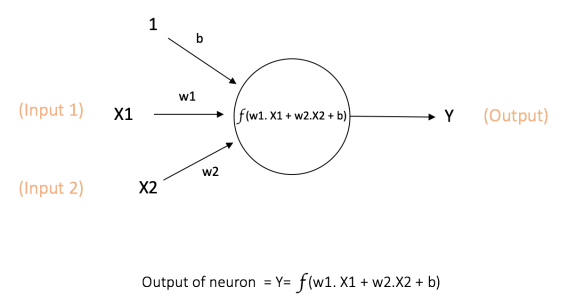
\includegraphics[scale=1.0]{perceptron}
  \caption{An example of a single Neuron}
  \label{fig:Perceptron}
\end{figure}
The network takes numerical inputs \textit{X1} and \textit{X2} and has weights \textit{w1} and \textit{w2} associated with those inputs.
Additionally, there is another \textit{input 1} with weight \textit{b} (called \textit{Bias}) associated with it. The main function of Bias is to provide every node with a trainable constant value (in addition to the normal inputs that the node receives). The output Y from the neuron
is computed as shown in the Figure \ref{fig:Perceptron}. The function \textit{f} is non-linear and is called \textbf{Activation Function}. The
purpose of the activation function is to introduce non-linearity into the output of a neuron. This is important because most real world data
are non linear and we want neurons to learn these non-linear representations.
\subsubsection{Activation Functions} 
Every activation function (or non-linearity) takes a single number and performs a certain fixed mathematical operation on it. There are
several activation functions:
\begin{description}
\item[ Sigmoid ] : takes a real-valued input and squashes it to range between 0 and 1. Its formula is:
  \[ \sigma(x) = \frac{1}{1 + e^{-x} } \]
  It is easy to understand and apply but it has major reasons which have made it fall out of popularity:
  \begin{itemize}
  \item Vanishing gradient problem
  \item Its output isn’t zero centered. It makes the gradient updates go too far in different directions.
  \item Sigmoids saturate and kill gradients.
  \item Sigmoids have slow convergence.
  \end{itemize}

\item [ Tanh ] : takes a real-valued input and squashes it to the range [-1, 1]. Its formula is:
  \[ tanh(x) = 2 \sigma(2x) -1 \]
  Now it’s output is zero centered because its range in between -1 to 1. Hence optimization is easier in this method and  in practice it is always preferred over Sigmoid function . But still it suffers from Vanishing gradient problem.

\item[ ReLU ]: ReLU stands for \textit{Rectified Linear Unit}. It takes a real-valued input and thresholds it at zero (replaces negative values with zero). So its formula is:
  \[ f(x) = max(0,x) \]
  It has become very popular in the past couple of years. It was recently proved that it had 6 times improvement in convergence from Tanh
  function. Seeing the mathematical form of this function we can see that it is very simple and efficient . A lot of times in Machine
  learning and computer science we notice that most simple and consistent techniques and methods are only preferred and are best.
  Hence it avoids and rectifies vanishing gradient problem . Almost all deep learning Models use ReLu nowadays.
\end{description}

Figure \ref{fig:Activation}  show each of the above activation functions.
\begin{figure}[h]
  \centering
  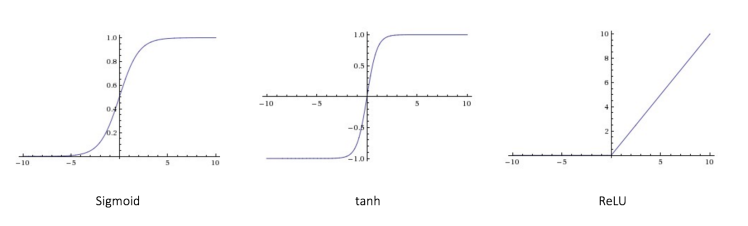
\includegraphics[scale=1.0]{activation_figures}
  \caption{Plots of Activation functions}
  \label{fig:Activation}
\end{figure}

\subsubsection{Feed-forward Neural Network}
Till now we have covered neuron and activation functions which together for the basic building blocks of any neural network. The feedforward
neural network was the first and simplest type of artificial neural network devised. It contains multiple neurons (nodes) arranged in layers.
A layer is nothing but a collection of neurons which take in an input and provide an output. Inputs to each of these neurons are processed
through the activation functions assigned to the neurons. Nodes from adjacent layers have connections or edges between them. All these connections have weights associated with them.
\begin{figure}[h]
  \centering
  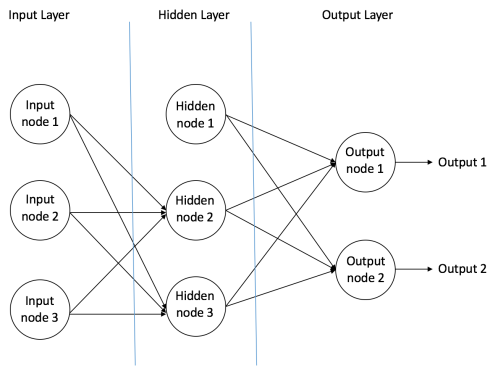
\includegraphics[scale=1.0]{feedforwardnetwork}
  \caption{An example of a Feedforward Neural Network}
  \label{fig:feedforwardnetwork}
\end{figure}
An example of a feedforward neural network is shown in Figure \ref{fig:feedforwardnetwork}. A feedforward neural network can consist of three types of nodes:
\begin{description}
\item[ Input Nodes ] The Input nodes provide information from the outside world to the network and are together referred to as the
  “Input Layer”. No computation is performed in any of the Input nodes – they just pass on the information to the hidden nodes.
\item[  Hidden Nodes ]  The Hidden nodes have no direct connection with the outside world (hence the name “hidden”). They perform
  computations and transfer information from the input nodes to the output nodes. A collection of hidden nodes forms a “Hidden Layer”.
  While a feedforward network will only have a single input layer and a single output layer, it can have zero or multiple Hidden Layers.
\item [ Output Nodes ] The Output nodes are collectively referred to as the “Output Layer” and are responsible for computations and
  transferring information from the network to the outside world.
\end{description}

In a feedforward network, the information moves in only one direction – forward – from the input nodes, through the hidden nodes (if any)
and to the output nodes. There are no cycles or loops in the network (this property of feed forward networks is different from Recurrent
Neural Networks in which the connections between the nodes form a cycle). Another important point to note here is that each of the hidden
layers can have a different activation function, for instance, hidden layer1 may use a sigmoid function and hidden layer2 may use a ReLU,
followed by a Tanh in hidden layer3 all in the same neural network. Choice of the activation function to be used again depends on the
problem in question and the type of data being used.

\subsection {2D Convolutional Neural Network}
A Convolutional Neural Network (ConvNet/CNN) is one of the variants of neural networks used heavily in the field of Computer Vision. It
derives its name from the type of hidden layers it consists of. The hidden layers of a CNN typically consist of convolutional layers, pooling
layers, fully connected layers, and normalization layers. Here it simply means that instead of using the normal activation functions defined
above, convolution and pooling functions are used as activation functions.
It can take in an input image, assigning importance (learning weights and biases) to various aspects/objects in the image and be able to
differentiate one from the other. The pre-processing required in a ConvNet is much lower as compared to the other classification algorithms.
While in primitive method filters are hand-engineered, with enough training, ConvNets have the ability to learn these filters/characteristics.

The architecture of a ConvNet is analogous to that of the connectivity pattern of Neurons in the Human Brain and was inspired by the
structure of the Visual Cortex. However, most ConvNets consist mainly in 2 parts:
\begin{description}[font=$\bullet$\scshape\bfseries]
\item [ Feature extractor] : \\
  This part of the network takes as input the image and extract features that are meaningful for its classification. It amplifies aspects
  of the input that are important for discrimination and suppresses irrelevant variations. Usually, the feature extractor consists of
  several layers. For instance, an image which could be seen as an array of pixel values. The first layer often learns representation
  that represent the presence or absence of edges at particular orientations and locations in the image. The second layer typically
  detects motifs by spotting particular arrangements of edges, regardless of small variations in the edge positions. Finally, the third
  may assemble motifs into larger combinations that correspond to paths of familiar objects, and subsequent layers would detect objects
  as combinations of these parts.
  
\item [ Classifier ] : \\
  This part of the network takes as input the previously computed features and use them to predict the correct label.
\end{description}

\begin{figure}[h]
  % 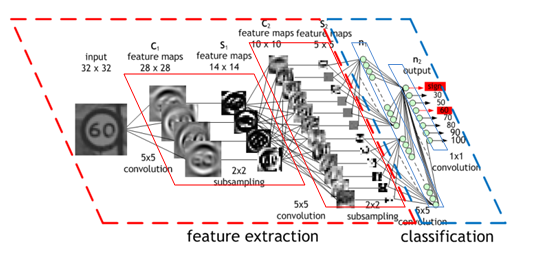
\includegraphics[scale=0.7]{convolutional_neural_network_structure} \]
  \centering
  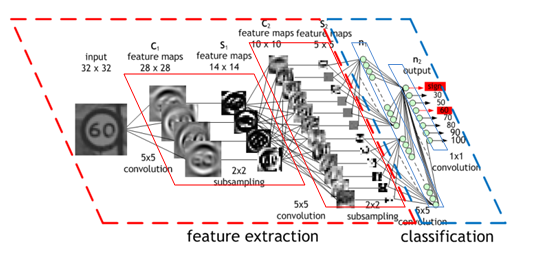
\includegraphics[scale=0.7]{convolutional_neural_network_structure}
  \caption{Typical structure of a ConvNet}
\end{figure}
\paragraph{Convolutional Layers}
In order to extract such features, ConvNets use 2D convolution operations. These operations take place in convolutional layers. Convolutional
layers consist of a set of learnable filters. Every filter is small spatially (along width and height), but extends through the full depth of
input. During forward pass, we slide (more precisely, convolve) each filter across the width and height of the input volume and compute dot
products between the entries of the filter and the input at any position (as Figure \ref{fig:conv_example} shows). The objective of the
Convolution Operation is to extract the high-level features such as edges, from the input image. ConvNets need not be limited to only one
Convolutional Layer. Conventionally, the first ConvLayer is responsible for capturing the Low-Level features such as edges, color, gradient
orientation, etc. With added layers, the architecture adapts to the High-Level features as well, giving us a network which has the wholesome
understanding of images in the dataset, similar to how we would.

\begin{figure}[h]
  \centering
  \begin{minipage}[b]{0.4\textwidth}
    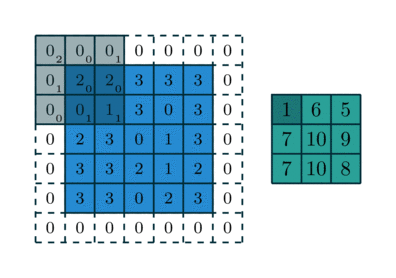
\includegraphics[width=\textwidth]{conv_1}
  \end{minipage}
  \hfill
  \begin{minipage}[b]{0.4\textwidth}
    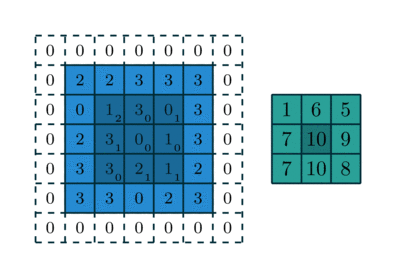
\includegraphics[width=\textwidth]{conv_2}
  \end{minipage}
  \caption{Convolution with kernel of 3, stride of 2 and padding of 1}
  \label{fig:conv_example}
\end{figure}
\paragraph{Pooling Layers}
Pooling Layers are also referred as downsampling layers and are used to reduce the spatial dimensions, but not depth, on a convolution neural network.
The intuitive reasoning behind this layer is that once we know that a specific feature is in the original input volume (there will be a high activation value),
its exact location is not as important as its relative location to the other features. The main advantages of pooling layer are:

\begin{itemize}
\item We gain computation performance since the amount of parameters is reduce.
\item Less parameters also means we deal with overfitting situations.
\end{itemize}

The pooling operation is specified, rather than learned. Two common functions used in the pooling operation are:
\begin{description}
\item[ Average Pooling ] Calculate the average value for each patch on the feature map.
\item[ Maximum Pooling (or Max Pooling) ] Calculate the maximum value for each patch of the feature map.
\end{description}

\begin{figure}[h]
  \centering
  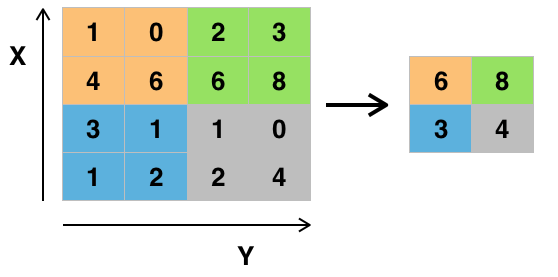
\includegraphics[scale=0.35]{max_pooling}
  \caption{Example of Max pooling operation with a 2x2 filter  and stride of 2}
  \label{fig:pooling_eg}
\end{figure}

\subsection{3D Convolutional Neural Network}
Traditionally, ConvNets are targeting RGB images (3 channels). The goal of 3D CNN is to take as input a video and extract features from it.
When ConvNets extract the graphical characteristics of a single image and put them in a vector (a low-level representation), 3D ConvNets
extract the graphical characteristics of a set of images. 3D CNNs takes in to account a temporal dimension (the order of the images in the
video). From a set of images, 3D CNNs find a low-level representation of a set of images, and this representation is useful to find the
right label of the video (a given action is performed). \\
In order to extract such features, 3D ConvNets  use 3D convolution operations.
\begin{figure}[h]
  % 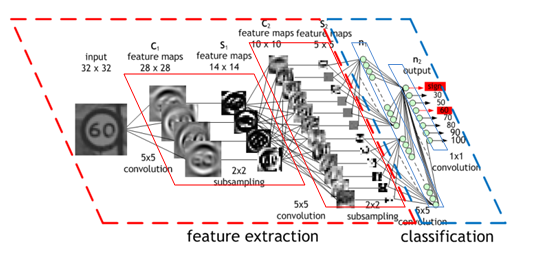
\includegraphics[scale=0.7]{convolutional_neural_network_structure} \]
  \centering
  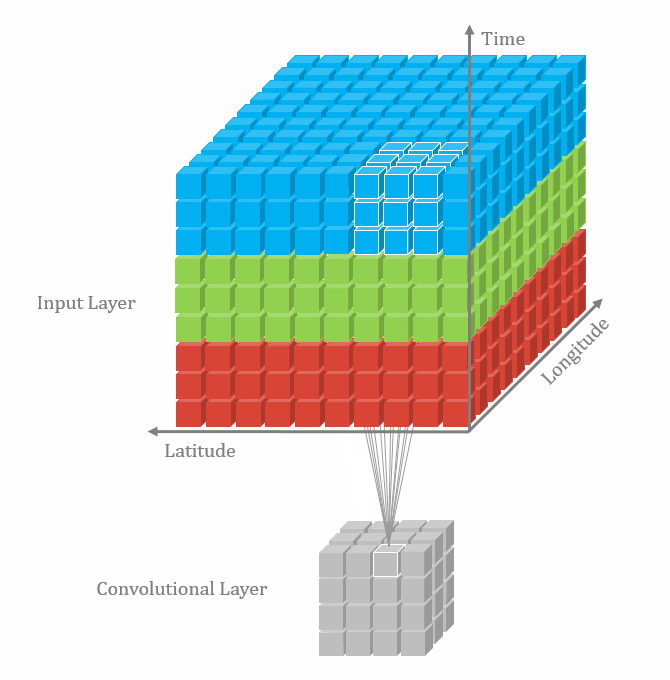
\includegraphics[scale=0.3]{3d_conv}
  \caption{3D Convolution operation}
\end{figure}

There are several existing approaches to tackle the video classification. This is a nonexaustive list of existing approaches:
\begin{description} [font=$\bullet$\scshape\bfseries]
\item[ ConvNets + LSTM cell] : Extract features from each frame with a ConvNet, passing the sequence to an RNN
\item[ Temporal Relation Networks] : Extract features from each frame with a ConvNet and pass the sequence to an MLP
\item[ Two-Stream Convolutional Networks] : Use 2 CNN, 1 spatial stream ConvNet which process one single frame at a time, and 1 Temporal stream ConvNet which process multi-frame optical flow
\end{description}

\section{Object Detection}
Within the field of Deep Learning, the sub-discipline called ``Object Detection'' involves processes such as identifying the objects through a picture, video or a webcam feed. The challenge of detecting all objects existing in image in countepart of action localization in videos and
a lot of object detection techniques are used in action localization architectures, so it is worth presenting it.
Object Detection methods are used almost everywhere these days. The use cases are endless such as Tracking objects, Video surveillance, Pedestrian detection etc. 
An object detection model is trained to detect the presence and location of multiple classes of objects. For example, a model might be trained with images that
contain various pieces of fruit, along with a label that specifies the class of fruit they represent (e.g. an apple, a banana, or a strawberry),
and data specifying where each object appears in the image.

The main process followed by most of CNN for Object Detection is:
\begin{enumerate}
\item Fistly, we do feature extraction using as backbone network, the first Convolutional Layers of a known pre-trained CNN such
  as AlexNet, VGG, ResNet etc.
\item Then, we propose regions of interest (ROI) in the image. These regions contain possibly an object, which we are looking for.
\item Finally, we classify each proposed ROI.
\end{enumerate}

\subsection{ Region Proposal Network}

From the 3 above steps, the 2nd step is considered to be very important. That is because, in this step, we should choose regions of
the image, which will be classified. Poor choice of ROIs means that the CNN will pass by some object that are located in the image,
because, they were not be proposed to be classified.

\begin{figure}[h]
  \centering
  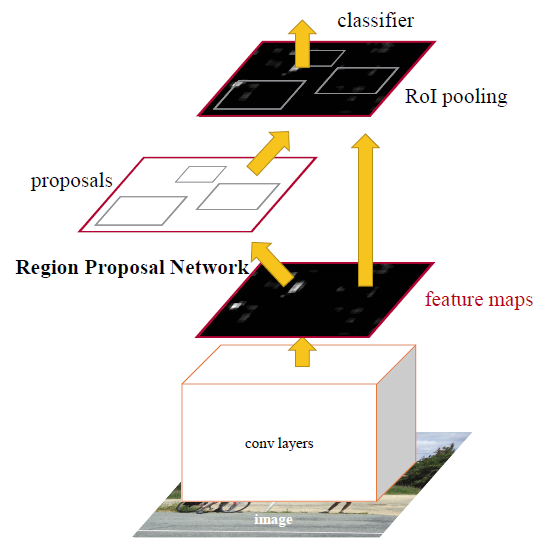
\includegraphics[scale=0.3]{RPN_structure}
  \caption{ Region Proposal Network's structure}
  \label{fig:rpn_structure}
\end{figure}

The first Object-Detection CNNs use several algorithms for proposing ROIs. For example, R-CNN(\cite{DBLP:journals/corr/GirshickDDM13}),
and Fast R-CNN(\cite{Girshick:2015:FR:2919332.2920125}) used Selective Search Algorithm for extracting ROIs.
One of novelties introduced by the Faster R-CNN(\cite{Ren:2015:FRT:2969239.2969250}) is \textbf{Region Proposal Network} (RPN). Its
function is to propose ROIs and its structure can be shown in \ref{fig:rpn_structure}. As we can see, RPN is consisted of:
\begin{itemize}
\item 1 2D Convolutional Layer
\item 1 score layer 
\item 1 regression layer
\end{itemize}

Before describing RPN's function, we introduce another basic element of RPN which is its \textbf{anchors}. Anchors are predefined boxes used for extracting ROIs. In figure \ref{fig:anchors} is
depicted an example of some anchors
\begin{figure}[h]
  \centering
  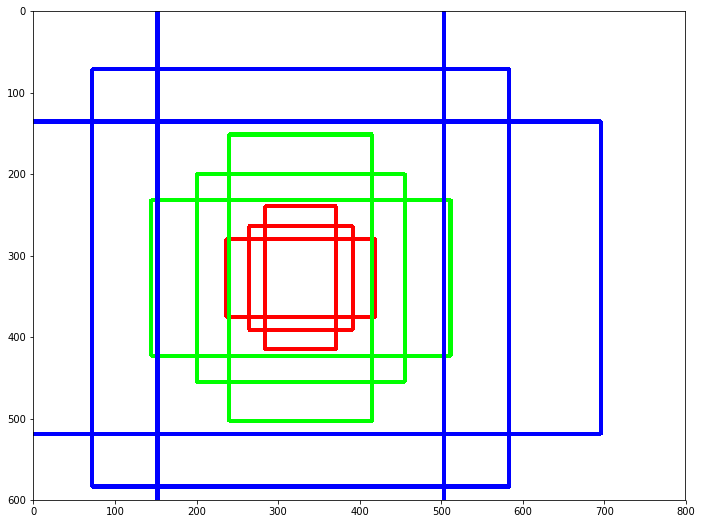
\includegraphics[scale=0.3]{anchors}
  \caption{ Anchors for pixel (320,320) of an image (600,800) }
  \label{fig:anchors}
\end{figure}

For each feature map's pixel corresponds \textbf{k (k=9)} anchors (3 different scales and 3 different ratios 1:1, 1:2, 2:1). \par
So, RPN's procedure is:
\begin{enumerate}
\item RPN gets as input feature maps extracted from the backbone CNN.
\item Then it performs 2D convolution over this input and passes the output to its scoring layer and regression layer.
\item Scoring layer produces confidence score of existing an object in each anchor's area. On the other hand, regression layer outputs 4k displacements, 4 for each anchor. Finally, we keep as output only the \textit{ n-best scoring} anchors.
\end{enumerate}

\subsection{Roi Align}

The biggest problem facing Object Detection Networks is the need for fixed input size. Classification networks require a fixed input size, which
is easy for image classification because it is handled by resizing the input image. However, in object recognition architectures, each proposal has a different size
and shape. This creates the need for converting all proposals to a fixed shape. At Fast-RCNN(\cite{Girshick:2015:FR:2919332.2920125}) and
Faster-RCNN(\cite{Ren:2015:FRT:2969239.2969250}) methods, this operation happens by applying Roi Pooling. However, this wrapping is digitalized because
the cell boundaries of the target feature map are forced to realign with the boundary of the input feature maps as shown in Figure \ref{fig:roi_pooling_align_1}
(the top left diagram). As a result, each target cells may not be in the same size (Figure \ref{fig:roi_pooling_align_2}).


\begin {figure}[h]

  \begin{subfigure}{0.35\textwidth}
    \centering
    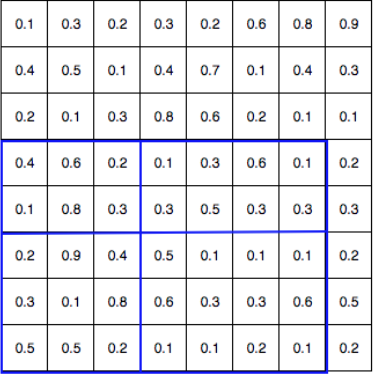
\includegraphics[scale=0.3]{roi_align_1}
    \caption{}
    \label{fig:roi_pooling_align_1}
  \end{subfigure}
  \hfill
  \begin{subfigure}{0.35\textwidth}
    \centering
    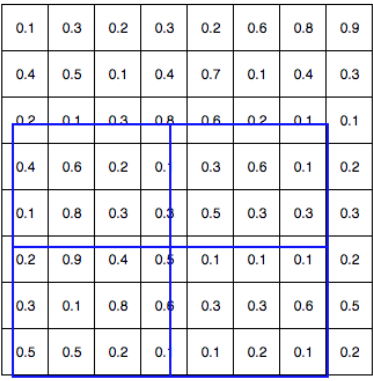
\includegraphics[scale=0.3]{roi_al_3}
    \caption{}
    \label{fig:roi_pooling_align_3}
  \end{subfigure}
  \hfill
  \begin{subfigure}{0.35\textwidth}
    \centering
    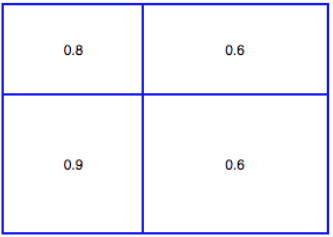
\includegraphics[scale=0.3]{roi_al_2}
    \caption{}
    \label{fig:roi_pooling_align_2}
  \end{subfigure}
  \hfill
  \begin{subfigure}{0.35\textwidth}
    \centering
    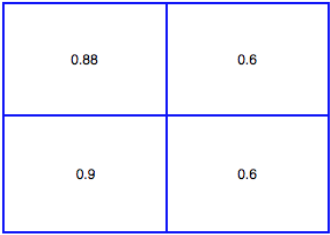
\includegraphics[scale=0.3]{roi_al_4}
    \caption{}
    \label{fig:roi_pooling_align_4}
  \end{subfigure}
  \caption{Roi Pooling and Roi Align examples}
  \label{fig:roi_pooling_align}
\end{figure}

On the other hand, Mask-RCNN (\cite{DBLP:journals/corr/HeGDG17}) introduced Roi Align operation. Roi Align avoids digitalizing
the boundary of the cells as shown in Figure \ref{fig:roi_pooling_align_3}, and achieves to make every target cell to have the same size
according to Figure \ref{fig:roi_pooling_align_4}. In order to calculate feature maps values, Roi Align uses bi-linear interpolation as
shown in Figure \ref{fig:roi_align_2}. This means that we calculate the value of the desired bins according to their neighbors'.

\begin{figure}[h]
  \centering
  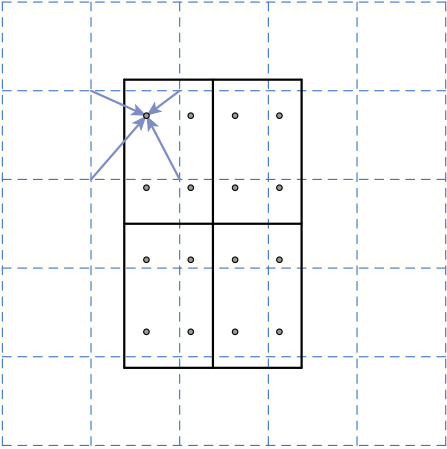
\includegraphics[scale=0.35]{roi_align_2}
  \caption{Example of bi-linear interpolation for calculation Roi Align's final feature map}
  \label{fig:roi_align_2}
\end{figure}

\subsection{Non-maximum suppression (NMS) algorithm}

Another problem that object detection networks face is that neighbourd bounding boxes have similar scores to some extent. Most object
detection systems employ a sliding window or a Region Proposal Network for proposing areas in the image that is likely to contain an
object. These techniques, which return several areas in the images, achieve high recall performance. However, in these approaches,
more that 1 proposal may be related with only one ground-truth object coordinates. This situation creates
the need for choosing the best proposals, because, alternatively, hundreds of unnecessary proposals will be classified. For that
reason, Non-Maximum Suppression (NMS) algorithm was proposed for filtering these proposals base on some criteria. NMS gets as input
a list of proposal bounding boxes B, their corresponding confidence score S and an overlap threshold N and return as output
a list of the final filtered proposals D. NMS algorithm's steps are:
\begin{enumerate}
  
\item Initialize an empty list D. Select the proposal with the highest confidence score, remove it from B and add it to D.
\item Calculate the overlap score between this proposal and all the other proposals. For all the proposals that their overlap
  score is bigger than N, remove from B.
\item From the remaining proposals, picked again the one with the highest score and remove it from B.
\item Repeat steps 2 and 3 until no more proposals are left in list B.
\end{enumerate}

The aforementioned algorithm shows that the whole process depends mostly on a single threshold value.  So that makes the selection
of threshold a crucial factor for the performance of the model. In some situations, bad choice of the threshold may make the network
to remove bounding boxes with good confidence score, if there are side by side. Figure \ref{fig:nms_eg} shows a situation like this,
where red and blue boxes will be removed because of the presence of the black box.
\begin{figure}[h]
  \centering
  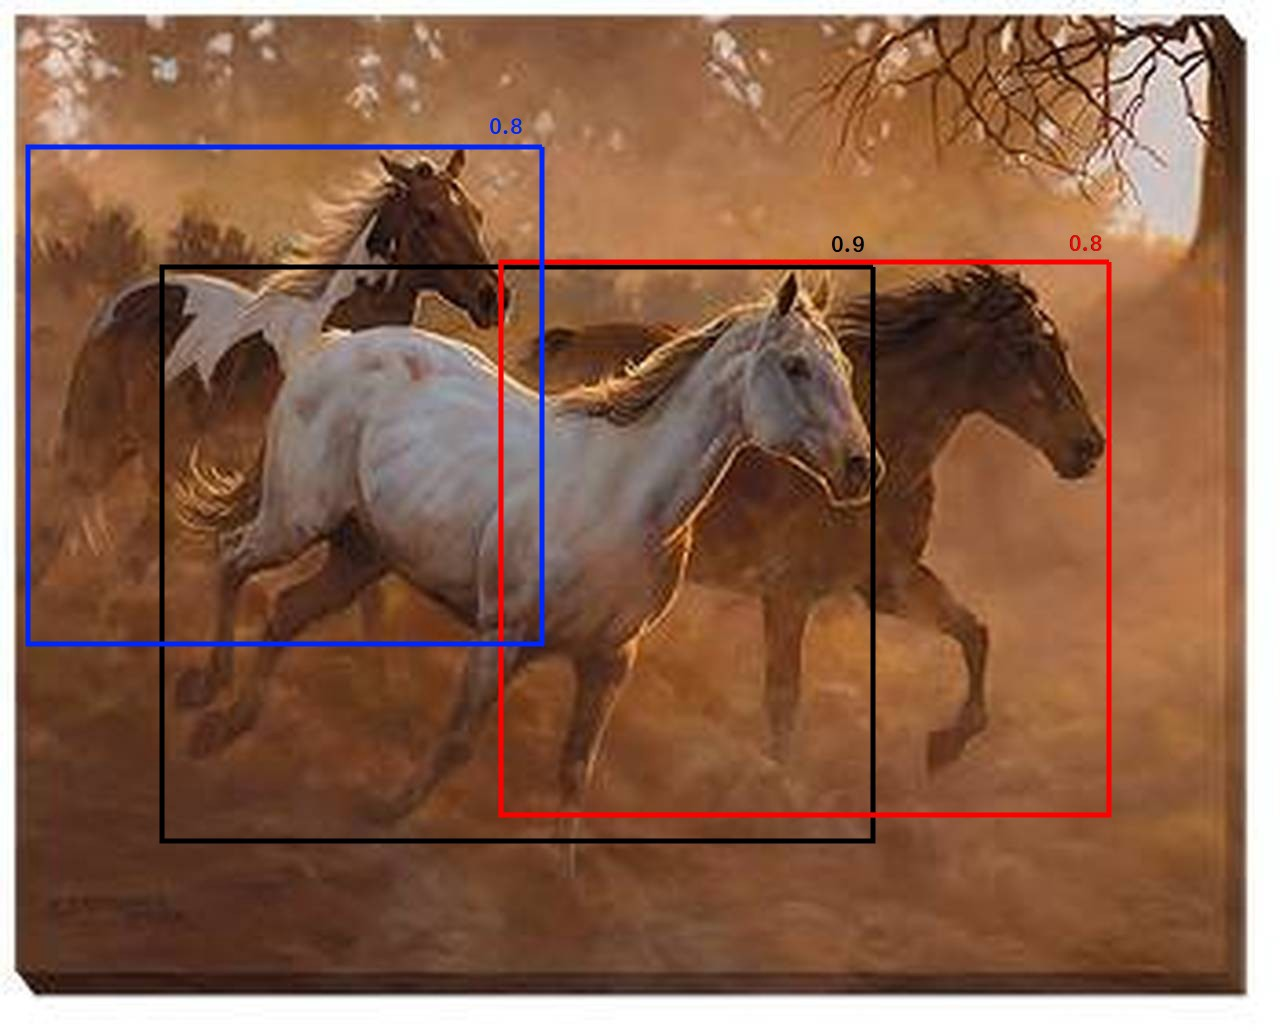
\includegraphics[scale=0.2]{soft_nms.jpeg}
  \caption{Example of a situation where NMS algorithm will remove good proposals}
  \label{fig:nms_eg}
\end{figure}

\subsubsection{Soft NMS}
A simple and efficient way to deal the aforementioned situation is to use Soft-NMS algorithm, which is presented in \cite{DBLP:journals/corr/BodlaSCD17}.
Soft-NMS algorithm is based on the idea of
reducing confidence score of the proposals proportional to their overlap score, instead of completely removing them.
The score calculation follows the formula 
\[ s_i = \begin{dcases}
    s_i, & overlapscore(M, b_i) < N_t \\
    s_i(1-overlapscore(M, b_i)), & overlapscore(M, b_i) \ge N_t
    \end{dcases}
    \]

    where $s_i$ is the score of proposal $i$, $b_i$ is the box coordinates of proposal $i$, $M$ is the coordinates of
    the box with the maximum confidence and $N_t$ is the overlap threshold. Let's, again, consider as input a list of
    proposal bounding-boxes B, their corresponding confidence score S and as output a list of proposals D. Soft-NMS algorithm includes the following steps:

\begin{enumerate}
  
\item Select the proposal with the highest confidence score, remove it from B and add it to D.
\item Calculate the overlap score between this proposal and all the other proposals. For all the proposals that their overlap
  score is bigger than N, recalculate their confidence score according to previous formula.
\item From the remaining proposals, picked again the one with the highest score and remove it from B.
\item Repeat steps 2 and 3 until no more proposals are left in list B.
\end{enumerate}
    
    
\section{Losses and Metrics}
In order to train our model and check its performance, we use some known Loss functions and Metrics used in Object Detection systems.
\subsection{Losses}
For training our network, we use \textbf{Cross Entropy Loss} for classification layers and \textbf{smooth L1-loss} for bounding box regression
in each frame and their diagram is show at Figure \ref{fig:cross_l1}.
\subsubsection{Cross Entropy Loss}
Cross-entropy loss, or log loss, measures the performance of a classification model whose output is a probability value between 0 and 1. \par
Entropy is the measure of uncertainty associated with a given distribution \textit{q(y)} and its formula is: 
\[ H = -\sum_{i=1}^n p_i \cdot \log p_i \]
Intuitively, entropy tells us how ``surprised'' we are when some event E happened. When we are sure about an event E to happened ($ p_E = 1$)
we have 0 entropy (we are not surprised) and vise versa. \par
On top of that, let's assume that we have 2 distributions, one known (our network's distribution) \textit{p(y)} and one unknown (the actual
data's distribution) \textit{q(y)}. Cross-entropy tells us how accurate is our known distribution in predicting the unknown distribution's
results. Respectively, Cross-entropy measures how accurate is our model in predicting the test data. Its formula is:
\[ H_p(q) = - \sum_{c=1}^C q(y_c) \cdot log(p(y_c)) \]

\subsubsection{Smooth L1-loss}

Smooth L1-loss can be interpreted as a combination of L1-loss and L2-loss. It behaves as L1-loss when the absolute
value of the argument is high, and it behaves like L2-loss when the absolute value of the argument is close to zero.
It is usually used for doing box regression on some object detection systems like Fast-RCNN(\cite{Girshick:2015:FR:2919332.2920125}),
Faster-RCNN(\cite{Ren:2015:FRT:2969239.2969250}) and it is less sensitive to outliers according according to \cite{Girshick:2015:FR:2919332.2920125}.
As shown in \cite{Girshick:2015:FR:2919332.2920125}, its formula is:

\[ smooth_{L1}(x) = \begin{dcases}
    0.5x^2 & \text{ if } x < 1 \\
    |x| - 0.5 & \text{otherwise}
  \end{dcases}\]

It is similar to Huber loss whose formula is:

\[
L_{\delta}(x) = \begin{dcases}
    \frac{1}{2}a^2 & \text{ for } |a| \le \delta \\
\delta(|a| - \frac{1}{2}\delta), & \text{otherwise}
\end{dcases}
\]

if we set $\delta $ parameter equal 1. \par

Smooth L1-loss combines the advantages of L1-loss (steady gradients for large values of \textit{x}) and L2-loss (less oscillations during
updates when \textit{x} is small). Figure \ref{fig:smooth_l1} shows a comparison between L1-norm, L2-norm  and smooth-L1 .

\begin{figure}[h]
  \centering
  \begin{subfigure}{0.49\textwidth}
    % \fbox{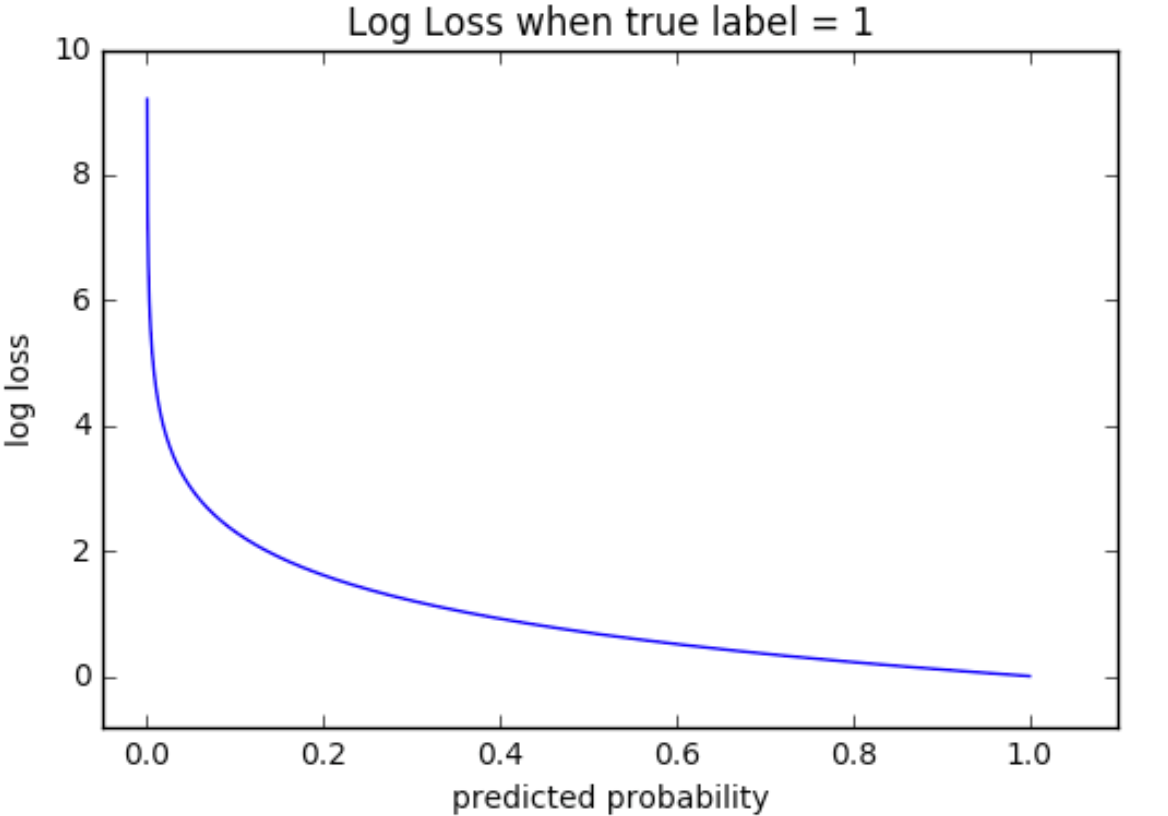
\includegraphics[width=\textwidth]{c_entropy}}
    % 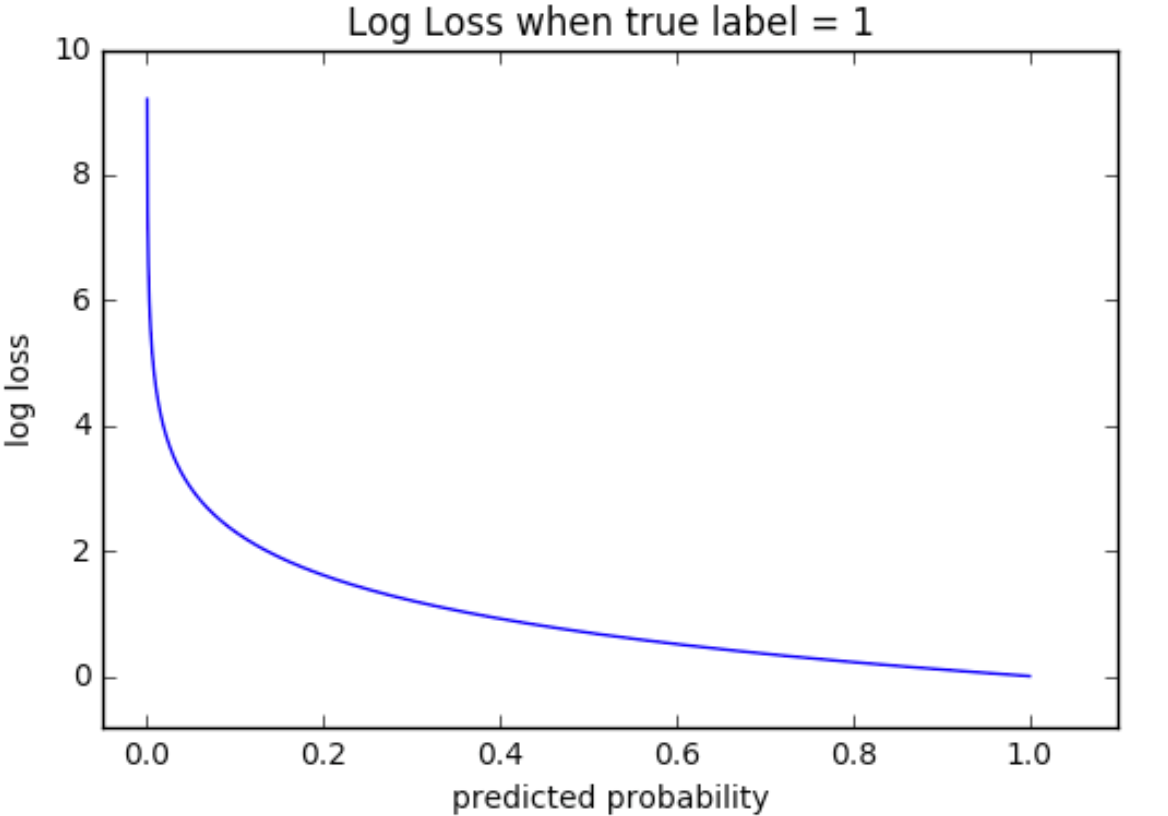
\includegraphics[width=\textwidth]{c_entropy}
    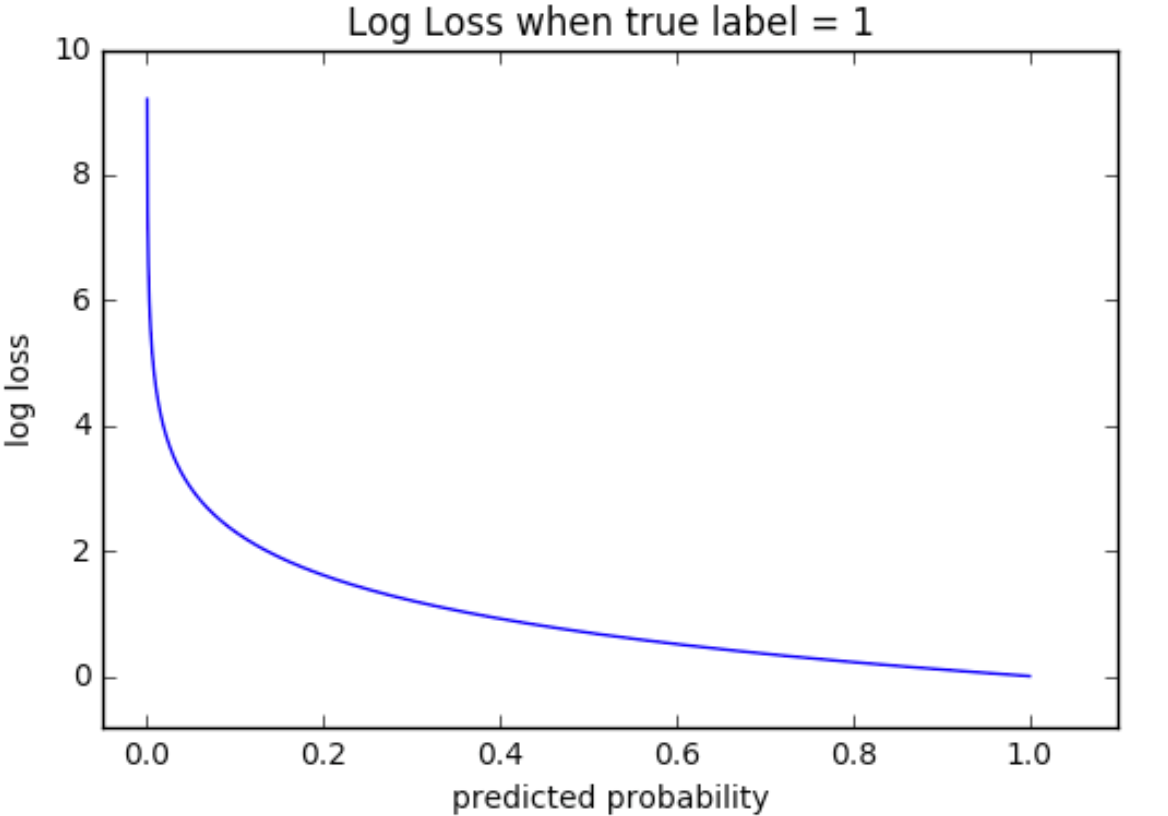
\includegraphics [width=7.0cm,height=4.5cm]{c_entropy}
      \caption{}
      \label{fig:cross_entropy}

  \end{subfigure}
  \hfill
  \begin{subfigure}{0.49\textwidth}
% \fbox{    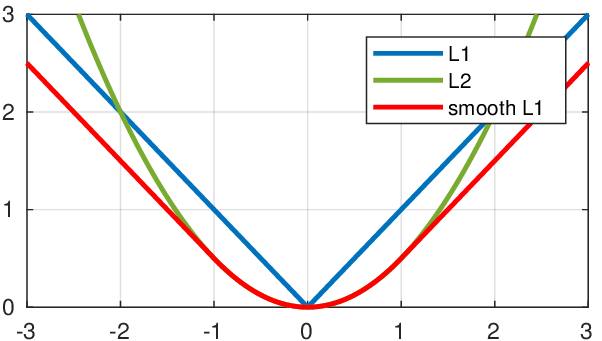
\includegraphics [width=5.5cm,height=3.8cm]{smooth_l1}}
    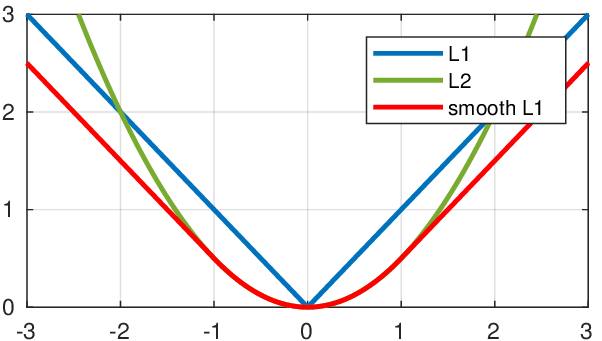
\includegraphics[width=\textwidth]{smooth_l1}
    % 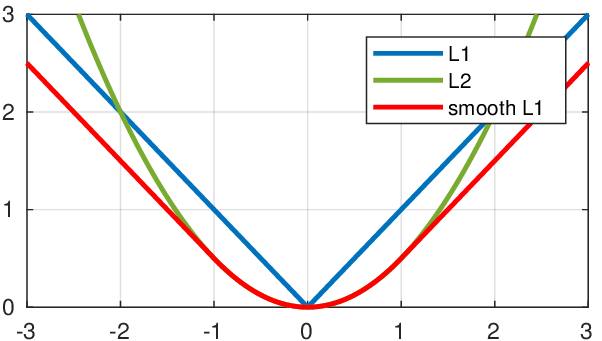
\includegraphics [width=6.0cm,height=4cm]{smooth_l1}
    % 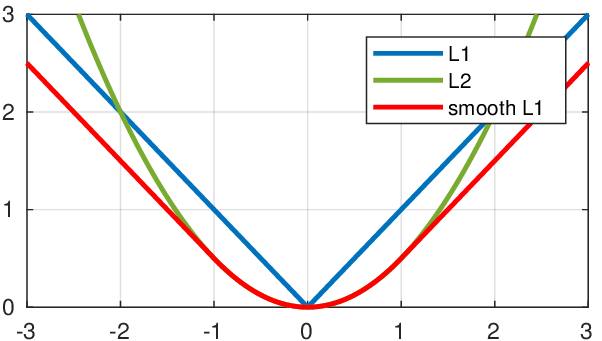
\includegraphics[width=\textwidth]{smooth_l1}
      \caption{}
      \label{fig:smooth_l1}
  \end{subfigure}

  \caption{ (\subref{fig:cross_entropy}) and (\subref{fig:smooth_l1})  show the behavior of cross-entropy loss and smooth-L1 respectively.}
  \label{fig:cross_l1}%
\end{figure}

\subsection{Metrics}
Evaluating our machine learning algorithm is an essential part of any project. The way we choose our metrics influences how the performance
of machine learning algorithms is measured and compared.
They influence how to weight the importance of different characteristics in the results and finally,
the ultimate choice of classification algorithm. Most of the times we use classification accuracy
to measure the performance of our model, however it is not enough to truly judge our model. \par
At first, we introduce some basic evaluation metrics in order,then, to present those we use for our assessment.

\subsubsection{Intersection over Union}
The first and most important metric that we use is Intersection over Union (IoU). IoU  measures the overlap between 2 boundaries.
It is usually used in Object Recognition Networks in order to define how good overlap a predicted bounding box  with the actuall
bounding box as shown in Figure \ref{fig:iou_fig}. We predefine an IoU threshold (say 0.5) in classifying whether the prediction is a true positive or a false positive.
\begin{figure}[h]
  \centering
  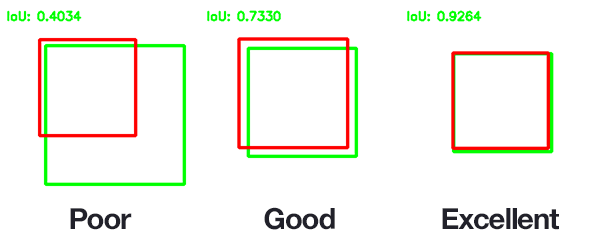
\includegraphics[scale=0.55]{iou}
  \caption{Example of IoU scoring policy}
  \label{fig:iou_fig}
\end{figure}

Intersection over Union is defined as:
\[ IoU = \frac{\text{area of overlap}}{\text{area of union}} \]
In Figure \ref{fig:iou_fig}, spatial IoU between 2 bounding boxes, $(x_1,y_1,x_2,y_2)$ and $(x_3,y_3,x_4,y_4)$,is presented, which means IoU metric is implemented for x-y dimensions.
Area of overlap and area of union can be defined as:
\[\text{ Area of overlap } = \lVert( min(x_2,x_4) - max(x_1,x_3), min(y_2,y_4)- max(y_1,y_3) )\rVert\]
\[\text{ Area of union  }  = \lVert( max(x_2,x_4) - min(x_1,x_3), max(y_2,y_4) - min(y_1,y_3) )\rVert\]
On top of that, we can implement IoU for 1 dimension and for 3 dimensions.
\paragraph{1D IoU} We can name 1D IoU as temporal overlap. Let's consider 2 temporal segments $(t_1,t_2)$ and $(t_3,t_4)$, between which we want to
estimate their overlap score. Their IoU can be described as:
\[ \text { Length of overlap } = \lVert(min(t_2,t_4) - max(t_1,t_3))\rVert  \]
\[ \text { Length of union } = \lVert(max(t_2,t_4) - min(t_1,t_3))\rVert  \]
\paragraph{3D IoU} 3-dimentional Intersection over Union which can, also, be named as spatiotemporal IoU, can be defined by 2 ways:
% categories: whether the $3^{rd}$ dimension is continuous or discrete.
\begin{description}
\item[3D boxes are cuboids] In this case, 3D boxes can be written  as $(x,y,z,x',y',z')$.
So, the IoU overlap between 2 boxes, $(x_1,y_1,z_1,x_2,y_2,z_2)$
  and $(x_3,y_3,z_3,x_4,y_4,z_4)$, is defined as:
\begin{equation*} 
\begin{split}
  \text { Volume of overlap } = \lVert(min(x_2,x_4) - max(x_1,x_3), \\
  min(y_2,y_4) -  max(y_1,y_3), min(z_2,z_4) -  max(z_1,z_3) ) \rVert  \\
\text { Volume of union } = \lVert(max(x_2,x_4) - min(x_1,x_3), \\
 max(y_2,y_4) - min(y_1,y_3), max(z_2,z_4) - min(z_1,z_3)
\end{split}
\end{equation*}

\item[x-y are continuous and z discrete] In this case 3D boxes is defined as a sequence of 2D boxes $(x,y,x',y')$. For this definition, z-dimension is
  discrete, and IoU can be defined with 2 ways, which both result in the same overlapping score. Let's cosider 2 sequences of boxes, with temporal limits
  $(t_1,t_2)$ and $(t_3,t_4)$. We calculate their IoU following one of the following methods:
  \begin{enumerate}
\item IoU is the product between temporal-IoU and the average spatial-IoU between 2D boxes in the overlapping temporal area and it is described as:
\[ IoU =  IoU((t_1,t_2),(t_3,t_4)) \cdot \frac{1}{K_2-K_1} \sum_{i=K_1}^{K_2} IoU(X_1^i, X_2^i) \]
  where \begin{itemize}
  \item$K_1 = min(t_2,t_4)$
  \item$K_2 = max(t_1,t_3)$
  \item$ X_1^i =  (x_1^i,y_1^i,x_2^i,y_2^i)$ and $X_2^i =  (x_3^i,y_3^i,x_4^i,y_4^i) $
  \end{itemize}
\item IoU is the average spatial-IoU if we consider 2D boxes as $(0,0,0,0)$ if $ t \notin [t_{start},t_{finish}]$ and it is written as:
  \[ IoU = \frac{1}{K} \sum_{i = min(t_1,t_3}^{max(t_2,t_4)} IoU(X_1^i,X_2^i) \]
  \begin{itemize}
  \item $K = max(t_2,t_4) - min(t_1,t_3)$
  \item $ X_1 = (x_1,y_1,x_2,y_2)  \text{ if } i \in [t_1,t_2] \text{ or }
        (0,0,0,0)  \text{ if } i \notin [t_1,t_2]  $
  \item $ X_2 = (x_3,y_3,x_4,y_4)  \text{ if } i \in [t_3,t_4] \text{ or }
        (0,0,0,0)  \text{ if } i \notin [t_3,t_4]  $
    \end{itemize}
  
\end{enumerate}
\end{description}
From above implementations, we are involve mostly with temporal and spatiotemporal IoU.

\subsubsection{Precision  \& Recall }

In order to describe \textbf{precision} and \textbf{recall} metrics, we will use an example. Let's consider a group of people in which, some of them are sick and
the others are not. We use a network which, given some data as input, is able to predict if a person is sick or not.
\begin{description}
\item[ Precision ]  measures how accurate are our model's predictions, i.e. the percentage of  predictions that are correct.
  In our case, how accurate is our model when it predicts that a person is sick.
\item[ Recall ] measures how well we found all the sick people. In our case, how many of the acctual sick people we managed to find.
\end{description}
Their definisions are:
\[ Precision = \frac{TP}{TP + FP} \]  
\[  Recall = \frac{TP}{TP + FN} \] 
where \begin{itemize}
\item TP = True positive, which means that we predict a person to be sick and he is actually sick.
\item TN = True negative, we predict that a person isn't sick and he isn't.
\item FP = False positive, we predict a person to be sick but he isn't actually.
\item FN = False negative, we predict a person not to be sick but he actually is.
\end{itemize}

From these 2 metrics we use recall metric in order to evaluate our networks performance, and more specifically, its performance on finding good action tube proposals.
We consider a groundtruth action as true positive when there is at least 1 proposed action tube that its IoU overlap score is bigger that
a predefined threshold. If there is no such action tube, then we consider this groundtruth action tube as false negative.


\subsubsection{mAP }

Precision and recall are single-value metrics based on the whole list of predictions. By looking their formulas, we can see that there is
a trade-off between precision and recall performance. This trade-off can be adjusted by the softmax threshold, used in model's final layer.
In order to have high precision performance, we need to decrease the number of FP. But this will lead to decrease recall performance and
vice-versa. \par
As a result, these metrics fail to determine if a model is performing well in object detection tasks as well as action detection tasks. For
that reason, we use mean Average Precision (mAP) metric, which for videos is named video-AP as introduced by \cite{DBLP:journals/corr/GkioxariM14}.
\paragraph{AP (Average precision)} Before defining mAP metric, we will define Average Precision metric (AP). AP is a popular metric in measuring the accuracy of
object detectors like Faster R-CNN, SSD, etc. Average precision computes the average precision value for recall value over 0 to 1.
As mentioned before, during classification stage, our prediction results in True positive(TP), False positive(FP), True Negative(TN) or False Negative(FN). For object recognition and action
localization networks, we don't care about TN. We consider a prediction as True positive when our prediction (an bounding box for object detection network or a sequence of bounding boxes in
action localization networks) overlaps with the groundtruth bounding box/action tube over a predefined threshold, and our predicted class is the same as groundtruth's. In addition, we
consider a False Negative when either no detection overlaps with the groundtruth bounding box/action tube or our prediction's class label was incorrect. We consider a prediction as False positive, when more that
one predictions overlap with the groundtruth. In this situation, we consider the prediction with the biggest confidence score as TP and the rest as FP.\par

For a class, we need to calculate, first, its precision and recall scores in order to calculate its AP score. We sort our predictions according to their confidence score and for each new prediction we
calculate precision and recall values. An example, for a class containing 4 TP and 8 predictions  is shown at Table \ref{table:map_1}. Precision and recall
are calculated according to the number of elements that are above in the order. So, for rank \#3, Precision is calculated as the proposion of TP = 2/3 = 0.67
and Recall as the proportion of TP out of all the possible TP = 2/4 = 0.5.

\begin{table}[h]
  \centering
  \begin{tabular}{|c | c | c | c |}
    \hline
    \textbf{Rank} & \text{Prediction} & \textbf{Precision} & \textbf{Recall} \\
    \hline
    1 & Correct & 1.0  & 0.25 \\
    \hline
    2 & Correct & 1.0  & 0.5 \\
    \hline
    3 & False   & 0.67 & 0.5 \\
    \hline
    4 & False   & 0.5  & 0.5 \\
    \hline
    5 & False   & 0.4  & 0.5 \\
    \hline
    6 & Correct & 0.5  & 0.75 \\
    \hline
    7 & False   & 0.42 & 0.75 \\
    \hline
    8 & Correct & 0.5  & 1   \\
    \hline
  \end{tabular}
  \caption{Ordered by confidence predictions and their precision and recall values}
  \label{table:map_1}
\end{table}

\begin{figure}[h]
  \centering
  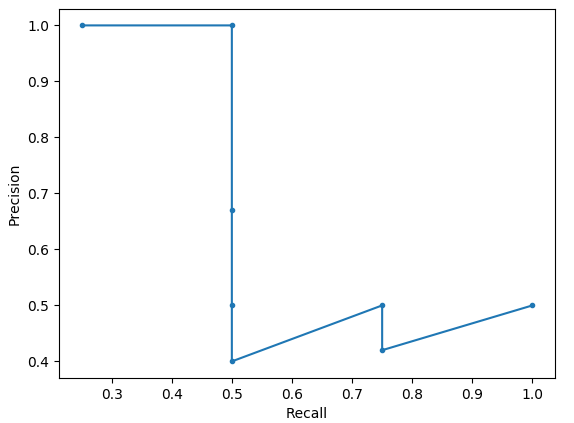
\includegraphics[scale=0.4]{pr_curve}
  \caption{Precision/Recall curve}
  \label{fig:pr_curve}
\end{figure}

We plot Precision against Recall and their curve is shown in Figure \ref{fig:pr_curve}.  The general definition for Average Precision(AP) is finding
the area under the precision-recall curve and its formula is:
\[ AP = \int_{0}^{1} p(r)dr \]
Precision and Recall values $ \in [0,1] $, so AP $\in [0,1]$, too. This integral can be replaced with a finite, as we have a finite number of predictions.
So its formula is:
\[ AP = \sum_{k=1}^{n} P(k)\Delta r(k) \]
where $P(k)$ is the precision until prediction $k$ and $\Delta r$ is the change in recall from $k-1$ to $k$.

\paragraph{Interpolated Precision}

As we can see at Figure \ref{fig:pr_curve}, P-R curve has a zigzag pattern as it goes down with false predictions, and goes up with correct.
So, before calculation AP, we need to smooth out this zigzag pattern using Intenpolated precision, as introduced in \cite{Everingham:2010:PVO:1747084.1747104}.
Interpolated precision is calculated at each recall level $r$ by taking the maximum precision measured for that $r$ and it is defined as:
\[ p_{interp}(r) = \max_{\tilde{r}:\tilde{r}\ge r} p(\tilde{r}) \]

where $p(\tilde{r})$ is the measured precision at recall $\tilde{r}$. Graphically, at each recall level, we replace each precision value
with the maximum precision value to the right of that recall level.  At Figure \ref{fig:pr_curve2} are shown both P-R curvers. The previous P-R curve has blue
colour and the interpolated has red colour.

\begin{figure}[h]
  \centering
  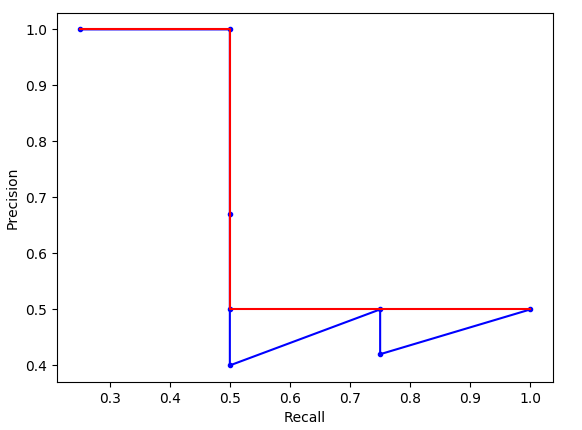
\includegraphics[scale=0.4]{pr_curve2}
  \caption{Both P-R curves. Interpolated P-R curve has red colour.}
  \label{fig:pr_curve2}
\end{figure}

In order to calculate AP, we sample the curve at all unique recalls values, whenever the maximum precision drops. On top of that, we define mean Average Precision (mAP)
the mean of the AP for each class. So, AP and mAP are defined as
\[  AP = \sum (r{n+1} - r_n) p_{interp} (r_{n+1}) \]
\[ p_{interp}(r_{n+1}) = \max_{\tilde{r} \ge r_{n+1} p(\tilde{r})}p(\tilde{r}) \]
\[ mAP = \frac{1}{N} \sum_{i=1}^N AP_i \]

\subsubsection{Mean Average Best Overlap - MABO}

In order to evaluate the quality of our proposals, both during TPN and connecting tube stages, recall metric isn't enough.
That's because recall metric tells us only for how many actual objects/action tubes, there was at least 1 proposal that satified the detection
criterion. However, it doen't tells us how close these proposals are to the actual objects/action tubes. In order to quantify this performance,
Mean Average Best Overlap (MABO) was introduced by \cite{DBLP:journals/corr/WinschelLE16}. The importance of MABO can be clarified 
we consider figure \ref{fig:mabo_fig}.

\begin{figure}[h]
  \centering
  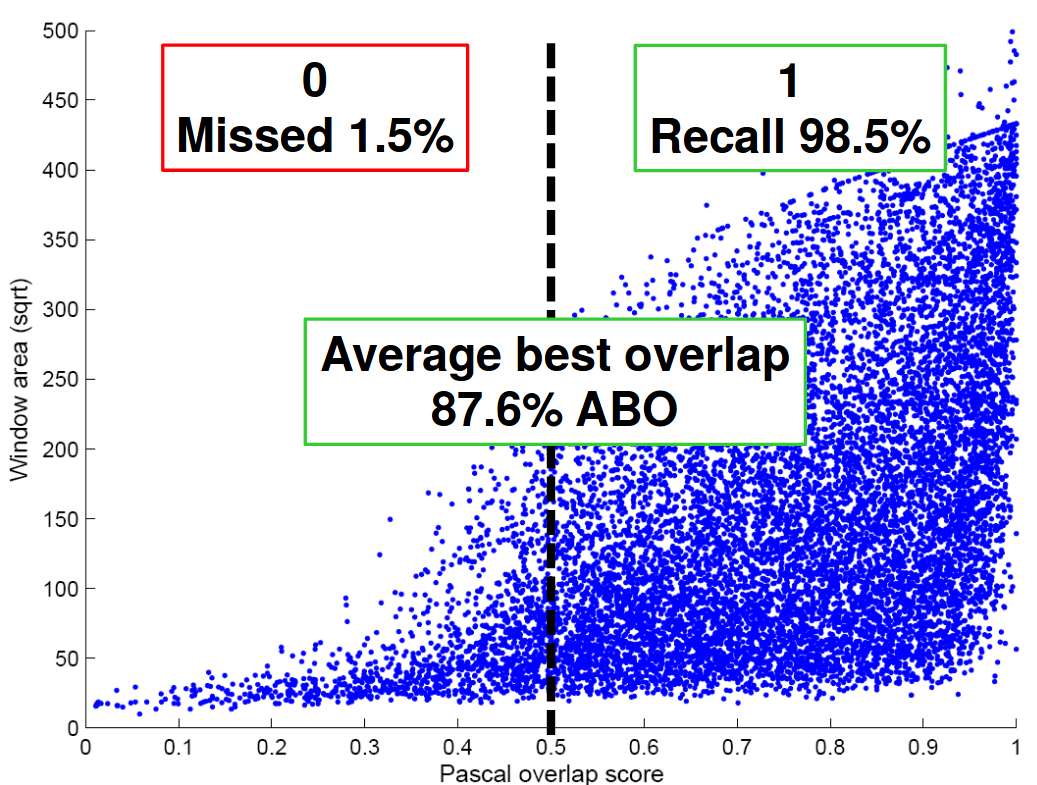
\includegraphics[scale=0.25]{mabo}
  \caption{Recall versus MABO exaple}
  \label{fig:mabo_fig}
\end{figure}

As we can see, recall performance is almost perfect, but, MABO perfonmance, which tells us where most proposal overlap scores are gathered,
is just fine and not perfect. \par
In order to define MABO, we need first to define Average Best Overlap. Let $ c \in C$ denote a class $c$ from the set of all
classes $C$ and $G^c$ the set of ground truth annotations of this class in all images; let $L$ be the set of all generated object proposals
for all images. Average Best Overlap is defined as the average value of the maximum overlap score, (in our situation, we use intersection
over union) of $L$ with each groundtruth annotation $g \in G^c$. The Mean Average Best Overlap (MABO) is defined as the average value of all
class ABO values :
\[ MABO = \frac{1}{|C|} \sum_{c \in C} [ \frac {1}{|G^C|} \sum_{g \in G^c} \max_{l \in L} IoU(g,l)]  \]
In our situation, which we care only for the quality of our proposals,  we consider only 1 class, foreground class. As a result, MABO's performance identifies with ABO's.

\section{Related work}
In this section, we present some of the most relevant methods to our work and others studied for designing this approach. These methods
 are divided into two sections: \textit{action recognition} and \textit{action localization}. The first part refers to classic action classification methods introduced until recently and the second part, respectively, to recent action localization methods. 
\subsection{Action Recognition}
First approaches for action classification consisted of two steps a) compute complex handcrafted features from raw video frames
such as SIFT, HOG, ORB features and b) train a classifier based on those features. These features can be seperated into 3 categories:
1) space-time volume approaches, 2) trajectories and 3) space-time feaures. For space-time volume methods the approach is as follows. Based on the training videos, the system contructs a 3D space-time model, by concatenating 2D images (x-y dimension) along time (t or z dimension),
in order to represent each action. When system is given an unlabeled video, it constructs a 3D space-time volume corresponding to this video.
This new 3D volume, then, is compared with each activity model to measure the similarity in shape and appearence between these two volumes.
The system extracts the class label of the unknown video by corresponding to the action with the highest similarity. Futhermore, there are
several variations of space-time representations. Instead of volume representation, the system may represent the action as trajectories
in space-time dimensions  or even more, the action can be represented as a set of features extracted from the volume or the trajectories.
Pure space-time volume representations include methods of comparing foreground regions of a person (i.e. silhouelttes) like \cite{BobickAaron}
did, comparing volumes in terms of their patches like \cite{1467296}.  \cite{4270510} method uses oversegmented volumes, automatically
calculating a set of 3-D XYT volume segments that corresponds to a moving human. \cite{4587727} proposed filters for
capturing volume's characteristics, in order to match them more reliably and efficiently. From the other hand, trajectory-based approaches
include representing an action as a set of 13 joint trajectories (\cite{1541250}) or using a set of \textit{XYZT}-dimensions joint trajectories
obtained from moving cameras (\cite{1541251}). Finally, several methods use local features extracted from 3-dimensional space-time volumes,
like extracting local features at every frame and concatenate them temporally (\cite{784616, 990935, 1544882}, extracting sparse
spatio-temporal local interest points from 3D volumes (\cite{1238378, 1570899, Niebles, 1467373, Ryoo2006})
These approaches made the choise of
features a signifact factor for network's performance. That's because different action classes may appear dramatically
different in terms of their appearance and motion patterns. Another problem was that most of those approaches make
assumptions about the circumstances under which the video was taken due to problems such as cluttered
background, camera viewpoint variations etc. A review of the techniques, used until 2011, is presented in \cite{Aggarwal:2011:HAA:1922649.1922653}. \par

Recent results in deep architectures and especially in image classification motivated researchers to train CNN networks for
the task of action recognition. The first significant attempt was made by \cite{6909619}. They design their architecture based on the best-scoring CNN
in the ImageNet competition. they explore several methods for fusion of spatio-temporal features using 2D operations mostly and 3D convolution only in slow fusion.
\cite{simonyan2014two}  used a 2 CNNs, one for spatial information and one for optical flow and combined them using late fusion.
They show that extacting spatial context from videos and motion context from optical flow can improve significantly action recognition accuracy.
\cite{DBLP:journals/corr/FeichtenhoferPZ16} extend this approach by using early fusion at the end of convolutional layers,  instead of late fusion which
takes places at the last layer of the network. On top that, they used a second network for temporal context which they fuse with the other network using late
fusion. Futhermore, \cite{DBLP:journals/corr/WangXW0LTG16} based their method on \cite{simonyan2014two}, too. They deal with the problem of capturing long-range
temporal context and training their network given limited training samples. Their approach, which they named Temporal Segment Network (TSN), seperates the input
video in K segments and a short snippet from each segment is chosen for analysis. Then they fuse  the extracted spatio-temporal context, making, eventually, their
prediction.
Most recently, \cite{DBLP:journals/corr/ZhangWWQW16} and \cite{DBLP:journals/corr/ZhuLNH17a} used two-stream approach, too. \cite{DBLP:journals/corr/ZhangWWQW16} replace optical flow with motion vector which can be obtained directly from compressed videos without extra calculation and feeding it to . \cite{DBLP:journals/corr/ZhuLNH17a} trained a CNN for calculating optical flow, calling it
MotionNet and use a temporal stream cnn for project motion information to action labels. Finally, they use late fusion through the weighted averaging of the prediction scores ofthe temporal and spatial streams. On the other hand, a novel approach was introduced by \cite{DBLP:journals/corr/abs-1711-01467} incoporating attension maps to give signifact improvement in action recognition performance \par 

Some other methods included a RNN or LSTM network for classification like \cite{DBLP:journals/corr/DonahueHGRVSD14}, \cite{DBLP:journals/corr/NgHVVMT15} and \cite{DBLP:journals/corr/MaCKA17}.  \cite{DBLP:journals/corr/DonahueHGRVSD14} address the challenge of variable lenghts of
input and output sequences, explointing convolutional layers and long-range temporal recursions. They propose a Long-term Recurrent
Convolutional Network (LRCN) which is capable of dealing with the tasks of action Recognition, image caption and video description. In order to classify a given sequence of frames, LRCN firstly gets as input a frame, and in particular its RGB channels and optical flow and predicts a class label. After that, it extracts video class by averaging label probabilities, choosing the most probable class.
\cite{DBLP:journals/corr/NgHVVMT15} firstly explore several approaches for temporal feature pooling. These techniques include handling video
frames individually by 2 CNN architectures: either AlexNet or GoogleNet, and consisted of early fusion, late fusion of a combination between
them. Futhermore, they propose a recurrnet neural Network architecture in order to consider video clips as a sequences of CNN activations.
Proposed LSTM takes an input the output of the final CNN layer at each consequentive video frame and after five stacked LSTM layers using a
Softmax classifier, it proposes a class label. For video classification, they return a label after last time step, max-pool the predictions
over time, sum predictions over time and return the max or linearly weight the predictions over time by a factor g, sum them and return the max.
They showed that all approaches are 1\% different with a bias for using weighting predictions for supporting the idea that LSTM becomes progressively more informed. Last but not least,  \cite{DBLP:journals/corr/MaCKA17} use a two-stream ConvNet for feature extraction and either a LSTM or convolutional layers over temporally-constructed feature matrices, for fusing spatial and temporal information. They use a ResNet-101 for
extracting feature maps for both spatial and temporal streams. They divide video frames in several segments like \cite{DBLP:journals/corr/WangXW0LTG16} did, and use a temporal pooling layer to extract distinguished features. Taken these features, LSTM extracts embedded features from all segments.
% A comparison between RNN networks and dilated convolutions is presented in \cite{DBLP:journals/corr/abs-1803-01271}, even though they don't refer at.\textbf{Pending... description}
\par
Additionally, \cite{Tran2014LearningSF} explored 3D Convolutional Networks (\cite{pmid:22392705}) and introduced C3D network which  has
3D convolutional layers with kernels $ 3 \times 3 \times 3$.
This network is able to  model appearence and motion context simultaneously using 3D convolutions and it can be used as a feature extractor, too.
Combining Two-stream architecture and 3D Convolutions, \cite{DBLP:journals/corr/CarreiraZ17} proposed
I3D network. On top of that, the authors emphasize in the advantages of transfer learning for the task of action recognition by repeating 2D pre-trained weights
in the 3rd dimension. \cite{DBLP:journals/corr/abs-1708-07632} proposed a 3D ResNet Network for action recognition based on Residual Networks (ResNet)
(\cite{DBLP:journals/corr/HeZRS15}) and explore the effectiveness of ResNet with 3D Convolutional kernels.
On the other hand, \cite{DBLP:journals/corr/abs-1711-08200}  based their approach on DenseNets(\cite{DBLP:journals/corr/HuangLW16a}) and extend
DenseNet architecture by using 3D filters and pooling kernels instead of 2D, naming this approach as DenseNet3D. Futhermore, they introduce
Temporal Transition Layer (TTL), which concatenates temporal feature-maps extracted at different temporal depth ranges and replaces DenseNet's
transition layer. On top of that \cite{DBLP:DibaFSKAYG18} introduced  a new temporal layer that models variable  temporal Convolution kernel depths.
Last but not least, \cite{DBLP:journals/corr/abs-1711-11248} experiment with several residual network architectures using combinations of 2D and 3D convolutional layer. Their purpose is
to show that a 2D spatial convolution followed by a 1D temporal convolution achieves state of the art classification performance, naming
this type of convolution layer as R(2+1)D. 
Recently \cite{Guo_2018_ECCV} proposed a framework which can learn to recognize a previous unseen 3D action class with only a few examples
by exploiting the inherent structure of 3D data through a graphical representation. A more detailed presentation for Action Recognition techniques used until 2018 is included in
\cite{DBLP:journals/corr/abs-1806-11230}.

\subsection{Action Localization}

As mentioned before, Action Localization can be seen as an extention of the object detection problem. Instead of outputing 2D bounding
boxes in a single image, the goal of action localization systems is to output action tubes which are sequences of bounding boxes that
contain an performed action. So, there are several approaches including an object-detector network for single frame
action proposal and a classifier. \par
The introduction of R-CNN (\cite{DBLP:journals/corr/GirshickDDM13}) achieve significant improvement
in the performance of Object Detection Networks. This architecture, firstly, proposes regions in the image which are likely to
contain an object and then it classifies them using a SVM classifier. Inspired by this architecture, \cite{DBLP:journals/corr/GkioxariM14}
design a 2-stream RCNN network in order to generate action proposals for each frame, one stream for frame level and one for optical flow.
Then they  connect them using the viterbi connection algorithm. \cite{DBLP:journals/corr/WeinzaepfelHS15} extend this approach, by performing
frame-level proposals and using a tracker for connecting those proposals using both spatial and optical flow features. Also their method performs
temporal localization using a sliding window over the tracked tubes. \par
\cite{peng:hal-01349107} and \cite{DBLP:journals/corr/SahaSSTC16} use Faster R-CNN (\cite{Ren:2015:FRT:2969239.2969250}) instead of RCNN
for frame-level proposals, using RPN for both RGB and optical flow images.
After getting spatial and motion proposals,\cite{peng:hal-01349107} fuse them exploring and from each proposed ROI, generate 4 ROIs in order to focus in specific
body parts of the actor. After that, they connect the proposal using Viterbi algorithm for each class and perform temporal localization by using a sliding window, with multiple
temporal scales and stride using a maximum subarray method. From the other hand, \cite{DBLP:journals/corr/SahaSSTC16} perform, too, frame-level classification. After that,
their method performs fusion based on a combination between the actioness scores of the appearence and motion based proposals and their overlap score. Finally, temporal localization
takes place using dynamic programming. \par
On top of that, \cite{singh2016online} and \cite{kalogeiton17iccv:hal-01519812} design their networks based on the Single Shot Multibox Detector \cite{DBLP:journals/corr/LiuAESR15}).
\cite{singh2016online} created an online real-time spatio-temporal network. In order their network to execute real-time,  \cite{singh2016online} propose a novel and efficient algorithm
by adding boxes in tubes in every frame if they overlap more than a threshold, or alternatively, terminate the action tube if for k-frames no box was added.  \cite{kalogeiton17iccv:hal-01519812}
designed a two-stream network, which they called ACT-detector, and introduced anchor cuboids. For K frames, for both networks, \cite{kalogeiton17iccv:hal-01519812} extract spatial
features in frame-level, then they stack these features. Finally, using cuboid anchors, the network extracts tubelets, that is a sequence of boxes, with their corresponding classification
scores and regression targets. For linking the tubelets, \cite{kalogeiton17iccv:hal-01519812} follow about the same steps as \cite{singh2016online} did. For temporal localization, they use
a temporal smoothing approach. \par

Most recently, YOLO Network (\cite{DBLP:journals/corr/RedmonDGF15}) became the inspiration for \cite{DBLP:journals/corr/abs-1903-00304} and
\cite{DBLP:journals/corr/abs-1802-08362}. In \cite{DBLP:journals/corr/abs-1903-00304}, concepts of progression and progress
rate were introduced. Except from proposing bounding boxes in frame level, they use YOLO together with a RNN classifier for extracting temporal information for the proposals.
Based on this information, they create action tubes, seperated into classes. Some other approaches include pose estimation like \cite{DBLP:journals/corr/abs-1802-09232} do.% , \cite{} and
% . In \cite{DBLP:journals/corr/abs-1802-09232} uses \textbf{pending description...}. \par
They proposed a method for calcualatin 2D and 3D poses and then they performed action classification. They use the diffferentiable Soft-argamax function for estimating 2D and 3D joints, because
argmax function is not differentiable. Then, for T adjacent poses, they create an image representation with time and $N_j$ joins as $x-y$ dimensions and having 2 channes for 2D poses and 3
channels for 3D poses. They use Convolutional Layers in order to produce action heats and then using max plus min pooling and a Softmax activation they perform action classification.
Most of aforementioned networks use per-frame spatial proposals and extract their temporal infomation by calculating optical flow. On the other hand, \cite{DBLP:journals/corr/HouCS17} design
an architecture which icludes proposal in video segment level, which they called Tube CNN (T-CNN). Video segment level means that the whole video is seperated into equal length video clips, and
using a C3D for extracting features, it returns spatio-temporal proposals. After getting proposals, \cite{DBLP:journals/corr/HouCS17} link the tube proposals by an algorithm based on tubes'
actioness score and overlap. Finally, classification operation is performed for the linked video proposals.

\printbibliography

\end{document}
\message{ !name(chapter2_3.tex) !offset(-856) }
